

\pagebreak

\section {Using emotionally adaptive interface to influence performance of e-learning sessions}


\subsection{Problem description}

In the context of an e-learning environment the learner is subject to their personal emotional state which could potentially change over time. This affects their performance and the overall effectiveness of a learning session. (citation needed). E-learning aims to help users learn about subjects in a quick and effective way. Information about a users emotional and physical state can be incorporated into lessons to provide the user with a more appropriate task or interface.

\subsection{Goals of the paper}

Depending on the task, most beneficial emotional states of the learner are high-arousal positive-valence (upbeat) and low-arousal negative valence (calm, serious) \cite{NEEDED}
Some tasks require one, some the other. ^{(elaborate)}
My assumption is that, knowing the nature of the task and the optimal emotional state, we can transition the learner into a more adequate mood that as a result would allow more efficient learning.

I would like to explore how performance and engagement on a certain task is dependent on their mood and the presented interface.
Furthermore to evaluate whether UI and UX techniques could be leveraged to influence these two variables.

%- test if 2 different interfaces (oriented for positive valence (colorful,joyful) and negative valence(strict, b/w) ) and 2 different moods (pos and neg) lead to different performance on a task. Condition the user to a mood before presenting with the task.

\subsection{Approach and methods}

With the help of body and environment trackers we can gather data about the learner and with some certainty algorithmically predict their emotional state. Another approach would be to ask the user for their current state. Both could be combined to enhance the prediction and tailor it for each particular user. Each user is individual, so this additional verification step can be useful to train the algorithm to the user.

I would like to form a study of task performance depending on 2 variables:
\begin{itemize}
	\item Interface version (2 versions)
	\item Target Mood (2 moods: negative valence, low arousal; positive valence, high arousal)
\end{itemize}

\begin{figure}
	\begin{center}
		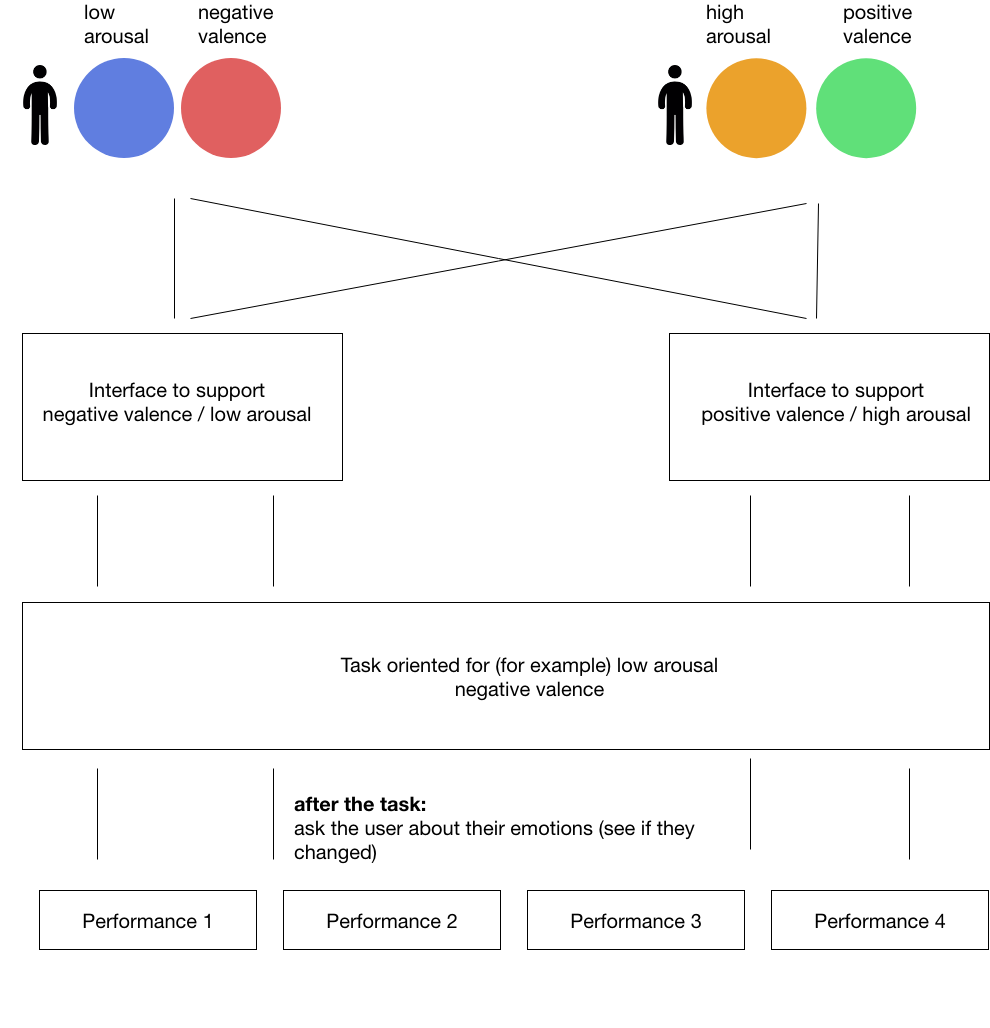
\includegraphics[width=0.5\textwidth]{images/study_design.png}
		\caption{Study design\label{fig:scaled_diss}}
	\end{center}
\end{figure}



First, I am planning to perform a quantitative analysis. Here a user would be presented with a choice of 2 interfaces and would perform the same task on both of them. Their mood shall be determined through a short questionnaire.
This would provide information if the same task can be accomplished more effectively with one of the provided interfaces. Both interface versions would provide the same usability features and should differentiate solely in the visual parameters that affect emotion (like use for color and language).

Further we might need to test if the same task is performed differently by the same user with the same interface but in two different moods. For this I would plan a more qualitative analysis with less test subjects and use preconditioning techniques to steer the user in a certain mood (video session, exercise session, different time of day). Their would perform the task on the same interface at two different points of time.

\subsubsection{Task}

Tasks can be different in nature, some of them require different mood states for optimal performance than others. The task for the study should be chosen carefully and based on previous studies proven to be best oriented for a specific mood.

Possibly find a standardized test to use (proven best for a certain kind of valence/arousal state)

\subsubsection{Measuring performance}

Performance can be measured in time spent, successful rate, mistakes per session etc.

\subsubsection{Interface}

Finding an interface that "fits" an emotion and supports it, as opposed to a neutral interface.

\subsubsection{Further thoughts}
Discuss viability of real-time or in-between-session measurement of mood to adjust interface taking in consideration the possibilities of current algorithms within LISA projects